% Template for APA submission with R Markdown

% Stuff changed from PLOS Template
\documentclass[a4paper,man,apacite,floatsintext]{apa6}
\usepackage{apacite}

% amsmath package, useful for mathematical formulas
\usepackage{amsmath}
% amssymb package, useful for mathematical symbols
\usepackage{amssymb}

% hyperref package, useful for hyperlinks
\usepackage{hyperref}

% graphicx package, useful for including eps and pdf graphics
% include graphics with the command \includegraphics
\usepackage{graphicx}

% Sweave(-like)
\usepackage{fancyvrb}
\DefineVerbatimEnvironment{Sinput}{Verbatim}{fontshape=sl}
\DefineVerbatimEnvironment{Soutput}{Verbatim}{}
\DefineVerbatimEnvironment{Scode}{Verbatim}{fontshape=sl}
\newenvironment{Schunk}{}{}
\DefineVerbatimEnvironment{Code}{Verbatim}{}
\DefineVerbatimEnvironment{CodeInput}{Verbatim}{fontshape=sl}
\DefineVerbatimEnvironment{CodeOutput}{Verbatim}{}
\newenvironment{CodeChunk}{}{}

% cite package, to clean up citations in the main text. Do not remove.
\usepackage{cite}

\usepackage{color}

% Use doublespacing - comment out for single spacing
%\usepackage{setspace}
%\doublespacing


% Text layout
\topmargin 0.0cm
\oddsidemargin 0.5cm
\evensidemargin 0.5cm
\textwidth 16cm
\textheight 21cm

% Bold the 'Figure #' in the caption and separate it with a period
% Captions will be left justified
\usepackage[labelfont=bf,labelsep=period,justification=raggedright]{caption}


% Remove brackets from numbering in List of References
\makeatletter
\renewcommand{\@biblabel}[1]{\quad#1.}
\makeatother


% Leave date blank
\date{}

%\pagestyle{myheadings}
%% ** EDIT HERE **


%% ** EDIT HERE **
%% PLEASE INCLUDE ALL MACROS BELOW

%% END MACROS SECTION


% ALL OF THE TITLE PAGE INFORMATION IS SPECIFIED IN THE YAML
\title{\textbf{Children's Processing of Ad-hoc Implicatures in Eye-tracking and Tablet
Studies}}
\shorttitle{Children's ad-hoc implicature processing}

\author{Erica J. Yoon, Michael C. Frank}

\affiliation{Department of Psychology, Stanford University}

\authornote{The Author Note, containing contact information, acknowledgements, etc}
\abstract{Language comprehenders routinely make pragmatic inferences that go
beyond the literal meanings of utterances. If A said ``I ate some of the
cookies,'' B should infer that A ate some \emph{but not all}. Children
perform poorly on experimental tests of scalar implicatures like this,
despite their early-emerging sensitivity to pragmatic cues. Our current
work explores potential factors responsible for children's successes and
failures in computing pragmatic inferences. In three experiments, we
used an eye-tracking paradigm (Experiments 1 and 2) and a tablet
paradigm (Experiment 3) to test children's ability to compute
implicatures when they have access to contextual alternatives to the
target word. We found that by the time children are four years old, they
successfully identify the inferential target referent in eye-tracking
and tablet paradigms. Younger children still struggle with computation
in our simplified tasks, however, and there is little evidence that this
struggle is caused by inhibitory demands of the tasks.}
\keywords{Pragmatics; implicature; eye-tracking; cognitive development}

\begin{document}
\maketitle

\section{Introduction}\label{introduction}

Language comprehension involves not only interpreting the literal
meanings of words in utterances, but also understanding the
communicative intentions behind what is said. Listeners make
\emph{pragmatic implicatures}, inferences about speakers' intended
meanings that go beyond the semantics of their utterances (Grice, 1975).
One common type of implicatures, called \emph{scalar implicatures},
involves scales built based on the knowledge of \emph{lexical}
alternatives (Horn, 1972). For example, if A says to B, ``Some of the
students failed the test,'' B may infer that A intended to say ``Some,
\emph{but not all}, of the students failed the test.'' That is, A's use
of the term ``some'' implicates that the stronger scalar alternative
``all'' is negated.

Whereas adults readily compute scalar implicatures (\emph{SI}s),
children tend to perform poorly on SI tasks (e.g., Noveck (2001),
Papafragou \& Musolino (2003), Huang \& Snedeker (2009)\}). For example,
given a context in which three out of three horses jumped over a fence,
adults reject a statement such as ``some of the horses jumped over the
fence'' as infelicitous, whereas children typically judge it to be
acceptable (Papafragou \& Musolino, 2003).

Children's failures on SI computation are surprising, given their
early-emerging sensitivity to the informativeness of utterances. For
example, by around approximately five years, children adjust
informativeness of their own expressions depending on the listeners'
knowledge (Matthews, Lieven, Theakston, \& Tomasello, 2006); reward
speakers based on their informativeness (Katsos \& Bishop, 2011); and
provide more information when disambiguation between potential referents
is difficult (Matthews, Butcher, Lieven, \& Tomasello, 2012). Given this
body of research, it seems unlikely that children's lack of pragmatic
ability per se causes their failures on SI tasks. What then causes
children's failures, and what factors can help them succeed on
implicature tasks?

One cue that may help children's implicature processing is availability
of alternatives to the current term. On standard accounts, implicature
involves generating and negating stronger alternatives to a given term.
Upon hearing ``some,'' the listener needs to generate a stronger
alternative (``all'') based on lexical knowledge, and then negate it.
One potential cause of children's difficulty with previous SI tasks
could be issues generating these alternative terms (Barner, Brooks, \&
Bale, 2011). If this hypothesis is true, children might succeed on
implicature computation if they are given access to alternatives in the
context.

Indeed, there is evidence that children can compute \emph{ad-hoc}
implicatures, which depend on contextually- rather than
lexically-derived scales (Stiller, Goodman, \& Frank, 2014).\footnote{These
  inferences are sometimes known in the pragmatics literature as
  ``particularized'' implicatures, in contrast to ``generalized''
  implicatures. Here we use the term ``ad-hoc'' implicature as a
  descriptive term and remain agnostic with respect to the reality of
  this distinction.} Children saw three faces, one wearing glasses and a
top-hat, one wearing glasses only, and one with no item. When children
heard: ``My friend has glasses,'' 3.5-year-old children and older chose
the face with glasses only as the referent above chance, successfully
computing the implicature ``My friend has glasses, \emph{but not a
top-hat},'' given the contextual access to the stronger alternative
(face with glasses and top-hat).

In the current work, we ask both about factors underlying the
previously-observed developmental trajectory and about the
decision-making processes underlying children's implicature computation.
In Experiment 1, we measure implicature performance across a wide
developmental range with an eye-tracking paradigm, and we replicate
Stiller et al. (2014)'s findings that preschoolers compute ad-hoc
implicatures. However, there are two surprising findings: younger
children (2- to 3-year-olds) consistently fail to compute implicatures
and are even more biased towards the wrong answer; and children's
performance in implicature trials is barely above chance, even for
5-year-olds. Experiments 2 and 3 address these concerns. In Experiment
2, we explore the cause of younger children's difficulty with
implicature computation and explore one potential cause: inability to
inhibit their response to more salient items. In Experiment 3, we use a
tablet paradigm to confirm children's robust implicature computation,
and compare their performances across the two methodologies used.

\section{Experiment 1}\label{experiment-1}

In Experiment 1, we use an eye-tracking paradigm to look at children's
ad-hoc implicature computation. Eye-tracking offers several advantages
over purely behavioral measures for examining pragmatic inference.
First, it is possible to track participants' gaze as an utterance is
being produced, providing moment-by-moment data about responses to
spoken language. Second, eye gaze reflects a more implicit measure of
comprehension and hence allows for more direct developmental comparisons
compared with behavioral choices that may reflect conscious
deliberation.

A previous eye-tracking paradigm looking at SI computation in children
(Huang \& Snedeker, 2009) suggested that children do not calculate SI
during online language processing. For example, when they saw a girl who
has two out of four (some but not all) of the socks and another girl who
has three out of three (all) of the soccer balls, and heard ``\ldots{}
the girl who has \emph{some} of the soc\ldots{},'' unlike adults,
children did not look more toward the girl with socks until they heard
the disambiguating word ``socks.'' Children might have struggled with SI
computation from the lack of access to lexical scales (some-all), and
the time constraint to process implicatures (in less than one second).
Our current work uses a similar but simpler paradigm that tests
children's inference of implicatures given scales that are set up
contextually.

Thus, in addition to replicating previous research on ad-hoc
implicatures in the online processing context, we are able to pursue two
goals in Experiment 1: measure the time-course of ad-hoc pragmatic
inference; and identify potential factors that contribute to the
developmental differences in implicature computation performance.

\subsection{Method}\label{method}

\subsubsection{Participants}\label{participants}

Parents and their 2- to 5-year-old children visiting Children's
Discovery Museum in San Jose, CA, were invited to participate in a short
video study. The current sample comprised of children who were exposed
to English at least 75\% of the time as indicated by their parents. In
addition, individual trials with more than 50\% missing gaze data were
excluded from analysis, and only participants who completed at least
half of the trials according to this criterion were included in the
analysis. These exclusion criteria led to a final sample of 123 (out of
143 participants): 26 2-year-olds (M = FIXME, range FIXME, FIXME girls),
33 3-year-olds (M = FIXME, range FIXME, FIXME girls), 29 4-year-olds (M
= FIXME, range FIXME, FIXME girls), 35 5-year-olds (M = FIXME, range
FIXME, FIXME girls). Children were given a sticker for participating in
the study. We also tested fifteen adult participants, undergraduate
students recruited through Stanford Psychology credit pool.

\subsubsection{Stimuli and Design}\label{stimuli-and-design}

On each trial, participants saw two images: a target and distractor,
which could either be an item with a single feature (e.g.~a plate with
only a carrot or only a banana), or an item with double features (e.g.,
a plate with a carrot and a banana). Each trial contained three phases:
in the initial phase (8.5 seconds), two images were presented in silence
for two seconds, then a pre-recorded voice said a sentence (e.g. ``Look
at these plates. Elmo's plate has a carrot.''). Then, in the
anticipatory phase (1.5 seconds), a chime sound played to induce
participants' anticipatory gaze. In the following feedback phase (1.5
seconds), a character appeared next to the target with an amusing sound
effect. This outcome served to keep the task engaging for participants.

There were three types of test trials (pictured in Figure FIXME). In
\emph{inference} trials, the target item had a single feature (e.g., a
carrot), and the distractor item had two features, one that was common
with the target (e.g., a carrot) and the other feature that was unique
(e.g., a banana). The test sentence named the feature that was common to
the target and distractor. Thus, if participants understood that
``Elmo's plate has a carrot'' implicates ``Elmo's plate has a carrot
\emph{but not a banana},'' given the context, they should look more
toward the target than the distractor, but otherwise look equally to
both.

There were two additional trial types, with semantically unambiguous
targets: \emph{Control-double} trials looked identical to inference
trials, but the target and distractor were switched, such that the
double-feature item was the target and the single-feature item was the
distractor, and the test sentence named the unique feature on the
target. \emph{Control-single} trials presented two items that each had a
unique single feature, and either could be the target. Children saw 4
inference, 4 control-double, and 4 control-single trials; adults saw 6
inference, 6 control-double, and 12 control-single trials.

There were six sets of item and feature types, and the features were
named with nouns found on the MacArthur-Bates Communicative Development
Inventory word list (Fenson et al., 1994). Two orders of the test trials
were created, such that trial types and item types were counterbalanced
and trial order was pseudo-randomized across the two orders.

\subsubsection{Procedure}\label{procedure}

Participants sat in a booster seat, approx. 60 cm away from the monitor
of an SMI RED 120 Hz binocular remote eye-tracker. Participants were
introduced to the task as watching a short video. The video began with a
short Elmo video clip that lasted for 1-2 minutes, during which any
necessary adjustments to the eye-tracker and participants' chair
positions were made. The eye-tracker was then calibrated using a 2-point
calibration and validation of the calibration points. Then participants
were introduced to Sesame Street characters and told ``Today, {[}they{]}
will show us lots of fun things. Are you ready? Let's go!'' Following
the introduction, participants saw two gaze-contingent practice trials,
with unambiguous targets that differed from the test items. Then
children watched 16 test trials and adults watched 24 test trials, as
well as 4 filler photos of children playing and 2 Elmo video clips,
presented at a pseudo-random points between test trials. The video
lasted approximately 8 minutes.

\subsection{Results and Discussion}\label{results-and-discussion}

\begin{CodeChunk}
\begin{figure}[tb]

{\centering 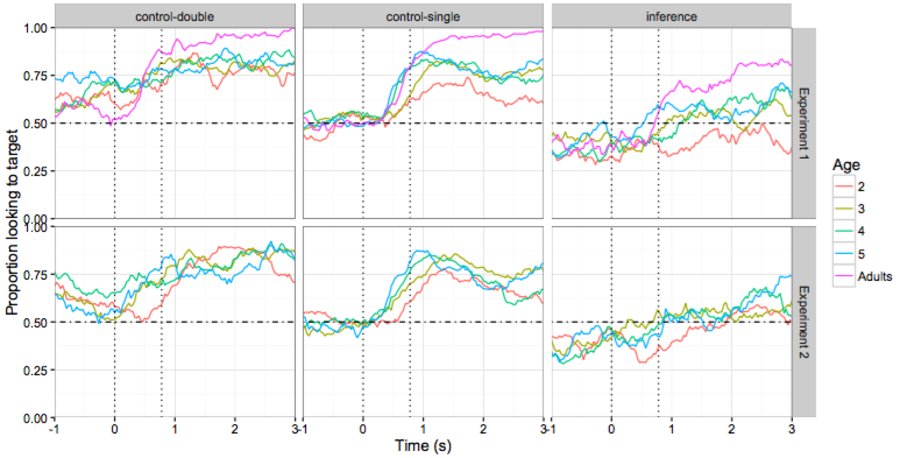
\includegraphics{figs/et_accuracy-1} 

}

\caption[Proportion of 2- to 5-year-old children and adults looking to the target image as the utterance unfolds]{Proportion of 2- to 5-year-old children and adults looking to the target image as the utterance unfolds. Time 0 represents the target word onset. Proportion correct looking is defined by looks to the target divided by the total looks to both the target and the distractor. (FIXME) Bottom panels show example stimuli from each condition; the named character emerged at the end of the trial to mark the correct target.}\label{fig:et_accuracy}
\end{figure}
\end{CodeChunk}

Participants of all ages looked to the targets in both control-double
and control-single trials reliably above chance (50\%; Figure 1). There
were age differences in the speed of looking at the target and the
proportion of correct looking across both control trial types.

For inference trials, children of 4 years and above robustly looked to
inferential targets (for 4-year-olds: \(t\)(28) = 2.55, \(p\) =0.016).
For example, upon hearing ``Bert's plate has a carrot,'' older children
identified the plate with only a carrot as the referent rather than the
plate with a carrot and a banana, replicating Stiller et al. (2014)'s
findings of ad-hoc implicature. Although previous studies are not
directly comparable due to low-level differences in the task and
materials, our finding is consistent with the hypothesis that children's
inferential ability might have been obscured in previous SI tasks due to
the unavailability of lexical alternatives (e.g. ``all'' given ``some'';
Barner et al. (2011)).

We additionally observed an unpredicted trend in two-year-olds'
behavior: they did not disengage from distractors relative to their
baseline bias prior to hearing the target word, and were marginally
\emph{below} chance in their overall performance (\(t\)(25) = -3.66,
\(p\) = 0.001). We address this issue in Experiment 2.

\begin{table}[tb]
\centering
\begin{tabular}{lrrr}
 Predictor & Estimate & Std. Error & $t$ value \\ 
  \hline
Intercept & 0.60 & 0.05 & 13.19 \\ 
  Control-double & 0.13 & 0.06 & 2.24 \\ 
  Inference & -0.33 & 0.06 & -5.24 \\ 
  Age & 0.04 & 0.01 & 3.34 \\ 
  Control-double * Age & -0.02 & 0.01 & -1.67 \\ 
  Inference * Age & 0.03 & 0.02 & 1.94 \\ 
   \hline
\end{tabular}
\caption{Predictor estimates with standard errors and significance information for a linear mixed-effects model predicting accurate looking to target in Experiment 1.} 
\label{tab:exp1_tab}
\end{table}

We fit a linear mixed-effects model\footnote{All mixed-effects models
  were run using the \texttt{lme4} package, version 1.1-10 (D. Bates,
  Maechler, Bolker, Walker, \& others, 2014). The random effects
  structure for this model was as follows:
  \texttt{(trial type \$\textbar{}\$ subid) + (age \$\textbar{}\$ item)}
  All of our data and processing and analysis code can be viewed in the
  version control repository for this paper at:
  \url{https://github.com/ejyoon/FIXME}.} to measure the effects of
trial type and age on the proportion of children looking to the target
between 0.8 and 4s after noun onset (Table 1). We selected this time
window because participants would have to wait until the end of target
noun (0.8 seconds on average) to know they should switch to the
inferential target, given the absence of a disambiguating continuation
(e.g., ``Elmo's plate has a carrot \emph{and banana}.''). Results of the
mixed-effects model indicate significant main effects of trial type and
age: participants looked to the target significantly less in inference
trials compared to control-single trials, and across all trial types,
participants' looking to target increased with age.

\begin{CodeChunk}
\begin{figure}[tb]

{\centering 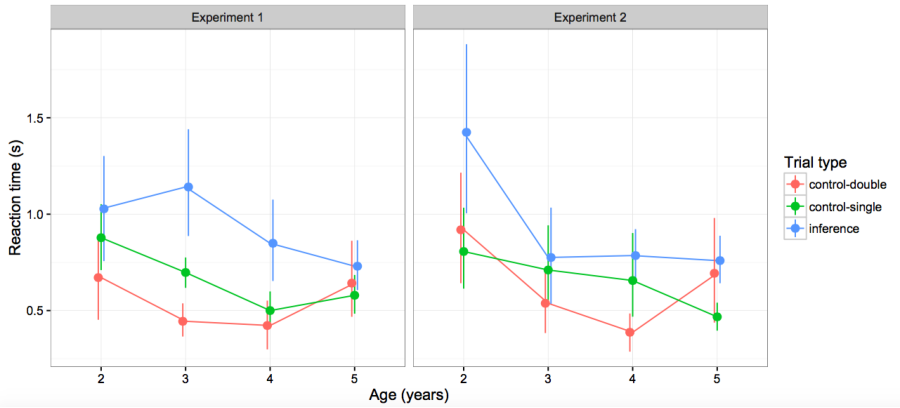
\includegraphics{figs/et_rt-1} 

}

\caption[Reaction times (time to switch from distractor to target) in Experiments 1 and 2]{Reaction times (time to switch from distractor to target) in Experiments 1 and 2}\label{fig:et_rt}
\end{figure}
\end{CodeChunk}

We next analyzed participants' reaction times (Fernald, Zangl, Portillo,
\& Marchman, 2008). We selected trials on which participants were
looking at the distractor at the point of disambiguation, and measured
the average length of time prior to a shift to the target. Looks to the
target were slower in inference trials compared to both control trial
types across all age groups (Figure 2). We next fit a linear
mixed-effects model with the same structure as the previous analysis,
but predicting reaction time rather than accuracy. This model again
showed significant main effects of trial type (\(\beta\) = 0.52,
\(p <.05\)) and age (\(\beta\) = -0.08, \(p <.01\)) on the average RT,
with no interaction (largest \(\beta\) = -0.06, \(p >.24\)). Inference
trials were generally slower compared to unambiguous control trials,
regardless of the participants' age, and participants reacted faster
with increasing age generally across trial types.

\section{Experiment 2}\label{experiment-2}

In Experiment 1, we largely replicated Stiller et al. (2014)'s findings
in an eye-tracking paradigm, and showed that adults and older children
(4- to 5-year-olds) look toward the pragmatically felicitous based on
ad-hoc implicature.

But younger children still struggled to look at the inferential target.
Further, 2-year-olds not only did not look at the correct inferential
target, but seemed to look if anything more toward the distractor. A
potential explanation for this pattern comes from the inhibitory demands
of our task. The two items in inference trials differed in salience:
Since the distractor item contained an extra referent (e.g., a carrot
and a banana), it was likely to be more salient. Supporting this idea,
looking to the two-referent item was greater than chance during the
baseline period of each trial. Perhaps 2- and 3-year-olds had difficulty
disengaging from this more salient (and logically possible) distractor
item in favor of the inferentially-correct target item. Inhibitory
control is difficult for children and continues to develop throughout
the period we studied here (e.g., Davidson, Amso, Anderson, \& Diamond
(2006)). In addition, several recent studies suggest that inhibitory
control might affect word recognition in similar eye-tracking paradigms
(Yurovsky \& Frank, 2014, Nordmeyer \& Frank (2013)).

Experiment 2 sought to explore the question of whether inhibitory
demands of the task caused younger children's failures. We increased the
saliency of distractor even more by presenting three instead of two
features.

\subsection{Method}\label{method-1}

\subsubsection{Participants}\label{participants-1}

Participants were recruited as in Experiment 1. The final sample
consisted of 102 (out of 126 participants): 26 2-year-olds (M = FIXME,
range FIXME, FIXME girls), 30 3-year-olds (M = FIXME, range FIXME, FIXME
girls), 36 4-year-olds (M = FIXME, range FIXME, FIXME girls), 27
5-year-olds (M = FIXME, range FIXME, FIXME girls).

\subsubsection{Stimuli}\label{stimuli}

The stimuli were identical to Experiment 1, except for one change:
target items in inference trials and distractor items in control-double
trials now had three features instead of two (see figure FIXME).

\subsubsection{Design and Procedure}\label{design-and-procedure}

The design and procedure were identical to Experiment 1.

\subsection{Results and Discussion}\label{results-and-discussion-1}

A linear mixed-effects model predicting accuracy based on age and trial
type in Experiment 2, as in Experiment 1, showed a significant main
effect of trial type (\(\beta\) = -0.25, \(p <.001\)), such that looking
at target was lower in inference trials than in control trials. There
was no significant main effect of age or interaction between age and
trial type (largest \(\beta\) = -0.25, \(p >.19\)). There was no
evidence of performance above \emph{or} below chance for any of the age
groups (largest \(t\): \(t\)(28) = 1.78, \(p\) =0.086)

A linear mixed-effects model looking at the reaction times of making
first switch from distractors to targets as in Experiment 1, found a
significant main effect of trial type (\(\beta\) = 0.58, \(p <.05\)) and
age (\(\beta\) = -0.1, \(p <.05\)) on the average RT, with no
interaction (\(\beta\) = -0.08, \(p >.23\)). Thus, participants' looking
was faster with increasing age, and looking at inferential targets was
slower and overall lower compared to unambiguous targets, consistent
with what was observed in Experiment 1.

\begin{table}[tb]
\centering
\begin{tabular}{lrrr}
 Predictor & Estimate & Std. Error & t value \\ 
  \hline
Intercept & 0.60 & 0.05 & 12.92 \\ 
  Experiment 2 & 0.07 & 0.07 & 1.00 \\ 
  Control-double & 0.13 & 0.06 & 2.11 \\ 
  Inference & -0.33 & 0.07 & -4.94 \\ 
  Age & 0.04 & 0.01 & 3.34 \\ 
  Experiment 2 * Control-double & 0.02 & 0.08 & 0.25 \\ 
  Experiment 2 * Inference & 0.08 & 0.10 & 0.86 \\ 
  Experiment 2 * Age & -0.02 & 0.02 & -1.28 \\ 
  Control-double * Age & -0.02 & 0.01 & -1.67 \\ 
  Inference * Age & 0.03 & 0.02 & 1.88 \\ 
  Experiment 2 * Control-double * Age & 0.00 & 0.02 & 0.13 \\ 
  Experiment 2 * Inference * Age & -0.02 & 0.02 & -0.79 \\ 
   \hline
\end{tabular}
\caption{Predictor estimates with standard errors and significance information for a linear mixed-effects model predicting accurate looking to target in Experiments 1 and 2.} 
\label{tab:exp2_tab}
\end{table}

\subsubsection{Comparison between Experiment 1 and
2}\label{comparison-between-experiment-1-and-2}

To determine the effect of saliency contrast on children's inferential
processing, we compared looking at targets across both Experiment 1 and
2 for inference trials. A linear mixed-effects model predicting accuracy
based on experiment, age, and trial type (Table 2) revealed significant
main effects of trial type and age, but no interaction between
Experiment 2 and any other variable. Thus, in contrast to our initial
predictions, we did not find evidence of the effect of perceptual
saliency on children's looking patterns. FIXME: post-hoc ana of
performance near end of the trials?

\section{Experiment 3}\label{experiment-3}

In Experiment 1, we confirmed that 4- and 5-year-olds reliably looked to
the pragmatically felicitous targets above chance, and thus saw evidence
of their implicature computation. Interestingly, however, the proportion
of looking to target was generally lower than expected, never reaching
beyond 75\%, whereas older children in Stiller et al. (2014)'s paradigm
selected the target much more robustly.

One potential source of this discrepancy is stimuli, in specific
pictures and utterances given. (FIXME: Add a point about how our task is
actually supposed to be easier?) Yet another important difference
between Stiller et al. (2014)'s and our paradigms is methodological one:
Stiller et al. (2014) used a behavioral selection paradigm on paper,
whereas we used an eye-tracking procedure. FIXME: selection paradigm
better estimate of children's accuracy, but eye-tracking offers us RT.
If looking time isn't the best to capture the rate at which children
make implicature computation, is there a paradigm that can show both
accuracy and reaction time, that are comparable to eye-tracking?

A tablet paradigm is a useful, engaging way to collect data from young
children, in that it yields comparable data to that of behavioral
paradigms, while making it possible to examine the accuracy and reaction
time of children's judgments (Frank, Sugarman, Horowitz, Lewis, \&
Yurovsky, 2016).

In Experiment 3, we examine children's ad-hoc implicature processing
using a tablet paradigm, and we revisit the findings from all
Experiments to compare the two methodologies, tablet vs.~eye-tracking.

\subsection{Method}\label{method-2}

\subsubsection{Participants}\label{participants-2}

Participants were recruited as in Experiment 1, except that a partial
sample was recruited from a local nursery school. The final sample
consisted of 62 (out of 64 participants): 24 3-year-olds (M = FIXME,
range FIXME, FIXME girls), 25 4-year-olds (M = FIXME, range FIXME, FIXME
girls), 13 5-year-olds (M = FIXME, range FIXME, FIXME girls).

\subsubsection{Stimuli}\label{stimuli-1}

FIXME: stimuli were presented on a tablet.

\subsubsection{Design and Procedure}\label{design-and-procedure-1}

FIXME: The design and procedure were identical to Experiment 2, except
that each participant saw all the possible numbers of features.

A linear mixed-effects model predicting accuracy based on age, trial
type and number of features present showed there was no significant main
effect or interaction (largest \(\beta\) = -0.12, \(p > .32\)).

A linear mixed-effects model predicting reaction time based on age,
trial type and number of features present showed no significant main
effect or interaction, other than a marginal main effect of age
(\(\beta\) = -321.44, \(p > .05\)).

\subsection{Comparing across Experiments 1, 2, and
3}\label{comparing-across-experiments-1-2-and-3}

\begin{CodeChunk}
\begin{figure}[tb]

{\centering 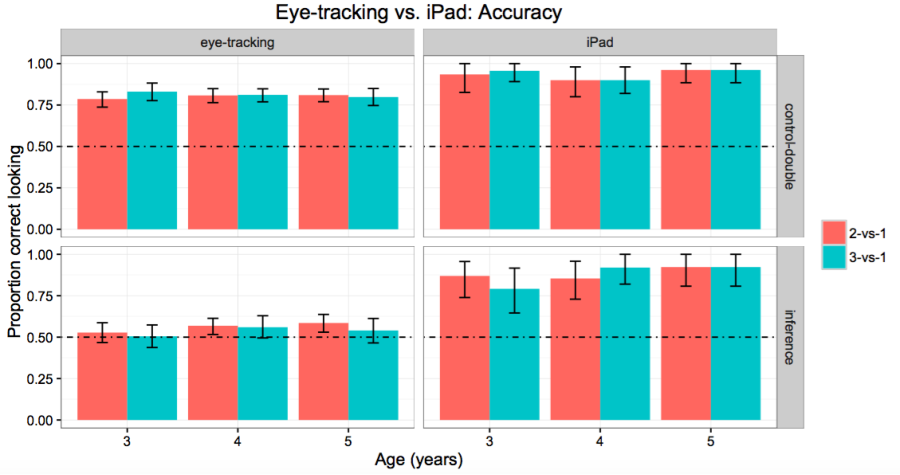
\includegraphics{figs/etip_accuracy-1} 

}

\caption[Accuracy rates across Experiments 1, 2 (eye-tracking), and 3 (iPad)]{Accuracy rates across Experiments 1, 2 (eye-tracking), and 3 (iPad). FIXME: change ylab}\label{fig:etip_accuracy}
\end{figure}
\end{CodeChunk}

\section{General Discussion}\label{general-discussion}

\newpage

\section*{References}\label{references}
\addcontentsline{toc}{section}{References}

Barner, D., Brooks, N., \& Bale, A. (2011). Accessing the unsaid: The
role of scalar alternatives in children's pragmatic inference.
\emph{Cognition}, \emph{118}(1), 84--93.

Bates, D., Maechler, M., Bolker, B., Walker, S., \& others. (2014).
Lme4: Linear mixed-effects models using eigen and s4. \emph{R Package
Version}, \emph{1}(7).

Davidson, M. C., Amso, D., Anderson, L. C., \& Diamond, A. (2006).
Development of cognitive control and executive functions from 4 to 13
years: Evidence from manipulations of memory, inhibition, and task
switching. \emph{Neuropsychologia}, \emph{44}(11), 2037--2078.

Fenson, L., Dale, P. S., Reznick, J. S., Bates, E., Thal, D. J.,
Pethick, S. J., \ldots{} Stiles, J. (1994). Variability in early
communicative development. \emph{Monographs of the Society for Research
in Child Development}, i--185.

Fernald, A., Zangl, R., Portillo, A. L., \& Marchman, V. A. (2008).
Looking while listening: Using eye movements to monitor spoken language.
\emph{Developmental Psycholinguistics: On-Line Methods in Children's
Language Processing}, 113--132.

Frank, M. C., Sugarman, E., Horowitz, A. C., Lewis, M. L., \& Yurovsky,
D. (2016). Using tablets to collect data from young children.
\emph{Journal of Cognition and Development}, \emph{17}, 1--17.

Grice, H. P. (1975). Logic and conversation. \emph{Syntax and
Semantics}, \emph{3}, 41--58.

Horn, L. R. (1972). \emph{On the semantic properties of logical
operators in english} (PhD thesis). University of California, Los
Angeles.

Huang, Y. T., \& Snedeker, J. (2009). Semantic meaning and pragmatic
interpretation in 5-year-olds: Evidence from real-time spoken language
comprehension. \emph{Developmental Psychology}, \emph{45}(6), 1723.

Katsos, N., \& Bishop, D. V. (2011). Pragmatic tolerance: Implications
for the acquisition of informativeness and implicature.
\emph{Cognition}, \emph{120}(1), 67--81.

Matthews, D., Butcher, J., Lieven, E., \& Tomasello, M. (2012). Two-and
four-year-olds learn to adapt referring expressions to context: Effects
of distracters and feedback on referential communication. \emph{Topics
in Cognitive Science}, \emph{4}(2), 184--210.

Matthews, D., Lieven, E., Theakston, A., \& Tomasello, M. (2006). The
effect of perceptual availability and prior discourse on young
children's use of referring expressions. \emph{Applied
Psycholinguistics}, \emph{27}(03), 403--422.

Nordmeyer, A. E., \& Frank, M. C. (2013). Measuring the comprehension of
negation in 2-to 4-year-old children. In \emph{Proceedings of the 35th
annual meeting of the cognitive science society}.

Noveck, I. A. (2001). When children are more logical than adults:
Experimental investigations of scalar implicature. \emph{Cognition},
\emph{78}(2), 165--188.

Papafragou, A., \& Musolino, J. (2003). Scalar implicatures: Experiments
at the semantics--pragmatics interface. \emph{Cognition}, \emph{86}(3),
253--282.

Stiller, A., Goodman, N. D., \& Frank, M. C. (2014). Ad-hoc implicature
in preschool children. \emph{Language Learning and Development}.

Yurovsky, D., \& Frank, M. C. (2014). Beyond naive cue combination:
Salience and social cues in early word learning. In \emph{Proceedings of
the 36th annual meeting of the cognitive science society}.

\bibliography{simpimp.bib}

\end{document}
